\chapter{Required Properties of E2E Systems\ifdraft{ (Dan) (60\%)}{}}
\label{chapter:required_properties}

We now describe the required properties that E2E VIV systems must have
in order to be considered for use in real elections. These
requirements can be broadly divided into two groups: \emph{technical
  requirements} and \emph{non-functional requirements}. Technical
requirements are those that can be directly addressed by the design
and implementation of the system, such as authentication requirements
for voters and election officials. Non-functional requirements are
those that are imposed on the system by external entities or where the
system depends on external behaviors outside its control, such as
specific election certification guidelines and operational
procedures. Each of these groups is itself divided into several
categories, and \autoref{fig:e2eviv_requirements_hierarchy} gives a
high-level overview of these.

\begin{figure}
\begin{center}
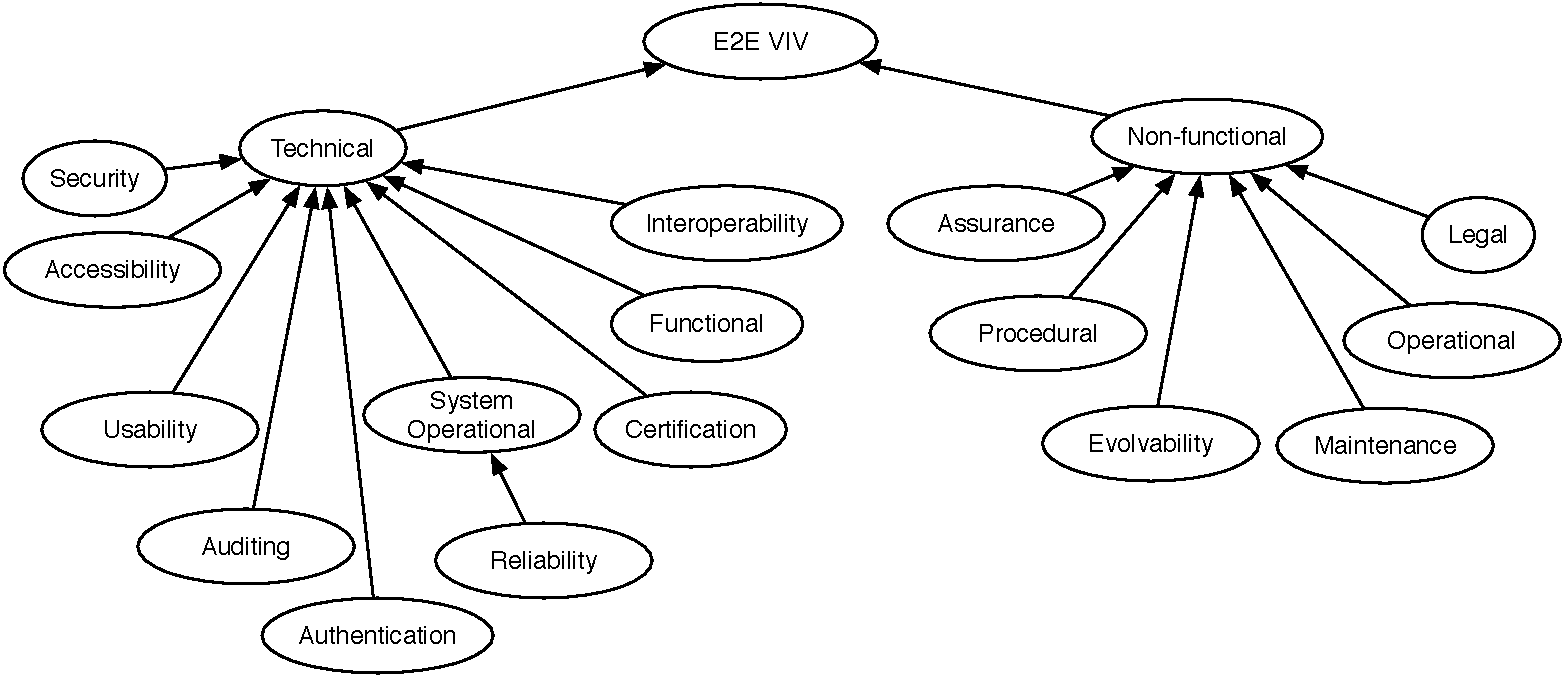
\includegraphics[width=6in]{required_properties_resources/hierarchy}
\end{center}
\caption{The hierarchy of requirements for E2E VIV systems.}
\label{fig:e2eviv_requirements_hierarchy}
\end{figure}

The following is a high-level description of the categories and many
of the requirements within each; \autoref{appendix:bon_requirements}
contains a complete listing of all E2E VIV system requirements
expressed in the Business Object Notation.\tododmz{is
  \autoref{appendix:bon_requirements} actually necessary, or will
  everything basically be described here?}

\section{Technical Requirements}
There are ten categories of technical requirements for E2E VIV
systems: functional, accessibility, usability, security,
authentication, auditing, system operational, reliability,
certification, and interoperability.

\subsection{Functional} 
\todogeneric{Should this really be ``functional''? Would ``core'' or
  something similar work better? It seems that some other
  requirements, such as those dealing with auditing and counting, are
  also functional...}  The functional requirements of an E2E VIV
system deal primarily with the casting and recording of ballots and
associated voter records. One important requirement is that there must
be a correspondence between the recorded ballots and the voters that
are listed as having voted; a ballot cannot be recorded without a
voter casting it, and a voter cannot be listed as having voted without
casting a ballot. Similarly, if a voter is informed by the system that
her ballot has been successfully cast, the system must correctly
retain the record of her having voted and her cast ballot information
even in the event of server failures.

Another functional requirement is the property of \emph{receipt
  freedom}: it must be impossible for a voter to prove to anybody any
information regarding how they voted their ballot, beyond what can be
mathematically deduced from the final distribution of votes. For
example, if a referendum passes with 100\% of the vote, there is no
way to hide the fact that every voter approved of the referendum;
however, if the result is mixed, it must be impossible for any
individual voter to prove how they voted. This must be the case even
when the voter can create digital evidence of her actions by, for
example, video recording the ballot casting process or photographing a
completed ballot.

In some elections voters are allowed to cast multiple ballots with
only the last cast ballot counting toward the final election tally,
while in others voters are prohibited from casting multiple
ballots. The system must accommodate both of these election formats,
ensuring that only the last cast ballot is counted for each voter when
multiple ballots are allowed and ensuring that each voter casts at
most one ballot otherwise.

Maintaining voter anonymity is critical, so it must be impossible
after the election to reconstruct a link between a cast ballot and any
identifying information about the voter who cast it. However, in
systems that support the casting of multiple ballots, it is important
to maintain links between voters and their ballots \emph{during} the
election to ensure that later ballots replace the correct earlier
ballots. To balance these concerns, it is a functional requirement of
the system that once it is determined that a ballot will be counted
toward the final tally, any link between that ballot and the voter who
cast it must be irrevocably broken.

Finally, because the voter should be able to focus on the voting
process without undue distractions or external influences, the voting
system must not display or permit the display of any advertising or
commercial logos during a voting session; the exception to this rule
is that an election jurisdiction may display its own logo to the voter
during the voting process. Along the same lines, the voting system
must not display any links to other Internet sites outside of the
voting system, except to provide help with the actual mechanics of
voting.

\subsection{Usability}

The usability of an E2E VIV system is critical to its successful
adoption and use. Since the user experience is so important, many of
the requirements of the system have some relation to usability even
though they may be categorized under other headings. There are,
however, two requirements that are exclusively related to the
usability of the system with respect to vote casting and one general
usability requirement that applies to the system as a whole.

The first vote casting requirement is that, if a voter receives a
final vote confirmation (e.g., ``Thank you for voting!'' or a similar
notice) from the system, she can be certain that her ballot was
recorded correctly. This is the usability counterpart to the
functional requirement that ballot records and voter records must be
maintained correctly even in the event of server failures.

The second vote casting requirement is that, if a voter is uncertain
whether or not her ballot was recorded (e.g., she clicked a ``submit''
button but never got a response from the system), she must be free
to attempt to vote again.

Finally, usability testing must be performed on any E2E VIV system
before it is deployed. The reports of the usability testing must be
made public, and the system must achieve satisfactory test results
before being used in a binding election.


\subsection{Accessibility}

Accessibility---the property of being usable by and useful to the
disabled---is one of the main goals of an E2E VIV system. It is
closely related to usability, but there are several requirements
associated specifically with accessibility that go beyond typical
usability requirements. 

Users must be involved in the design of the system to identify
accessibility constraints at each stage of the development
process. Consideration must be given to the system's compatibility
with existing technologies designed to help disabled individuals; for
example, the system should be developed in a way that allows assistive
input devices such as switches and eye trackers to be used in addition
to keyboards, mice and touchscreens. Similarly, the system's
presentation of voting options should be optimized to voters' needs by
providing alternative display fonts, audio representations, braille
representations, and other representations as appropriate.

All possible measures must be taken to ensure that the system can be
used by all voters and, if that is not possible in all circumstances,
to provide access to alternative methods of voting for those voters
who cannot use the system.

Finally, accessibility testing must be performed in addition to the
previously-mentioned mandatory usability testing. The reports of the
accessibility testing must be made public, and the system must achieve
satisfactory test results before being used in a binding election.

\subsection{Security and Authentication}

Security and authentication are closely related and together represent
the broadest set of technical requirements, consisting of both
requirements on the E2E VIV system itself (data storage,
communications, etc.) and requirements on the voting and counting
processes enabled by the system (voter authorization, voter privacy,
tally accuracy, etc.).

It is crucial that data integrity be ensured throughout the
system. Therefore, measures must be taken to ensure that no data can
be permanently lost in the event of a breakdown or fault affecting the
system; that the system maintains the integrity of the voters'
register, lists of candidates, ballot information, cast ballots, and
other critical information, in addition to authenticating the original
source(s) of that information and tracking provenance where
appropriate; that all data communications within the system have
associated integrity checks; that system equipment under the control
of the electoral authority is protected against influences that could
modify the election results; and that the integrity of the election
results does not depend in any way upon the security of system
equipment not under control of the electoral authority. The system
must perform regular ``health checks'' to ensure that data integrity
has been maintained, that all its components are operating in
accordance with their specifications, and that all system services are
available.

Accurate timing information is critical to security, both in terms of
providing evidence of compliance with applicable regulations, and in
terms of detecting attacks on and potential breaches of the
system. The system must therefore maintain reliable synchronized time
sources, with sufficient accuracy to maintain timing data for audit
trails, election observation data, and time limits for various aspects
of the election process. It must be possible to determine, using the
timing information stored by the system, whether nominations (and, if
required, acceptance thereof by the candidate or electoral authority),
voter registration, and vote casting have occurred within the
prescribed time limits for those actions.

Authentication and authorization are also important aspects of
security. The system must ensure that each individual can be
identified uniquely, so that there is no possibility of mistaking one
individual for another. The system must also maintain the privacy of
individuals, by ensuring that all personally identifiable data be kept
confidential as far as is allowed by the legal requirements of the
electoral jurisdiction. The system must allow access to each of its
services only to authorized users; for example, only individuals who
represent the electoral authority may be allowed to load ballot
information into the system.

The authentication mechanisms used to gain access to the system must,
as far as possible, protect authentication secrets (passwords,
one-time access codes, biometrics, etc.) so that unauthorized entities
cannot acquire them. Authentication to the E2E VIV system may not be
carried out through third parties; that is, existing online accounts
such as those at Facebook, Google and Twitter may not be used as
authentication mechanisms. The security of the authentication system
must not be affected by any potential breach of any public or
commercial database (e.g., a credit card database, the Social Security
database), and it should not be possible for an attacker to
impersonate a voter even if the entire database used for
authentication in the E2E VIV system is compromised. Individual
authentication secrets themselves must be changeable or revokable at
any time, at the behest of either the individual or election
officials, and must be changed for all individuals at least once in
every election cycle.

With respect to the actual voting process, only eligible voters may be
allowed to cast ballots and the system must ensure that only the
appropriate number of ballots is cast by each voter. It must be
possible for a voter to verify that the system has presented her with
an authentic ballot and, in the case of remote voting, that she has a
secure connection to an official server. 

The privacy of the vote must be preserved end-to-end to the maximum
extent possible, and individual voters may not waive the privacy of
their votes. In the case of remote voting, vote privacy must be
preserved even in the presence of arbitrary malicious code on the
voter's computer (corrupted client software, key logging software or
devices, etc.). Any client software used in remote voting must not
send data to any Internet host except those associated with the E2E
VIV system or provide any information to third parties (e.g.,
Facebook, Twitter, etc.) regarding the act of voting. Any residual
information that could be used to discover a voter's choices must be
destroyed after a ballot has been cast; if a voter uses a computer
outside the control of the electoral authority to cast her vote, she
must be provided with instructions for destroying any such information
on that computer.

With respect to vote counting, the system must accurately count the
votes and the counting process must be reproducible. The system must
also maintain the availability and integrity of all information used
to generate the final tally and all information regarding the counting
process itself for as long as required. 

Finally, it is expected that a deployed E2E VIV system will be an
attractive target for highly-capable adversaries that wish to
influence election results or to disrupt election processes. With this
in mind, the system must be designed and tested assuming that an
adversary has a budget of US\$10 per voter per election that can be
applied toward any critical subset of votes or voters of their
choosing; thus, an E2E VIV system for use in a U.S. presidential
election would need to be designed and tested assuming that an
adversary has a budget of approximately US\$1,300,000,000.

The electoral authority shall have overall responsibility for
compliance with these security requirements, and such compliance shall
be assessed by independent bodies as appropriate.

\subsection{Auditing}

The ability to perform comprehensive audits of system activity is one
of the important distinguishing aspects of an E2E VIV system as
compared to other voting systems; as a result, there are several
system requirements related specifically to auditing, in addition to
those security requirements (such as the tracking of accurate timing
information) that touch on auditing.

First, the audit system must be designed and implemented as part of
the E2E VIV system from the beginning; it cannot be added as an
afterthought to an existing system. Audit and monitoring facilities
must be integrated into all levels of the system, from low-level
communications among individual computers to high-level interactions
with election officials. The system must keep audit logs of all
activity relevant to the conduct and outcome of the election, and
these logs must be unmodifiable once they are written. These logs must
be as complete as possible without violating voter privacy.

The audit system must actively report on potential issues and threats,
rather than merely serving as a passive repository of system logs. It
must record at least the following events and actions with accurate
timing information: all voting-related information, including the
number of eligible voters and votes cast, the number of invalid votes,
count and recount results, etc.; any detected attacks on the operation
of the system or its communication infrastructure; and any system
failures, malfunctions, or other detected threats to proper system
operation. It must provide sufficient information to election
observers in real time, and after the election's conclusion, to verify
that the election is carried out in accordance with applicable
law.

The audit system must also be able to cross-check and verify the
correct operation of the voting system and the accuracy of the
election results, to detect voter fraud, and to prove that all counted
votes are legitimate and that all ballots have been counted. In
situations where the system cannot verify the legitimacy of all the
votes, it must be capable of giving an upper bound on the number of
affected ballots. If a tradeoff must be made between maintaining voter
privacy and identifying the perpetrators of fraud, the system must
resolve that tradeoff in favor of voter privacy.

In order for an E2E VIV system to be trusted, its auditability must
extend to its own source code as well as the activities it performs
during an election. Therefore, the E2E VIV system software, including
any official monitoring and auditing applications, must be published
in source form along with documentation, instructions for building and
running, and a digital signature as a proof of authenticity.

\subsection{System Operational}

System operational requirements ensure that the system is configured,
updated, and run in a transparent, accountable way that allows for the
other requirements to be fulfilled. One important such requirement is
that there must be official published manifests of the system used to
run any election, indicating details of the software and versions
used, dates of installation, and brief descriptions of their
functionality. Both public and private manifests must be maintained;
these should be identical, except that details about software used
solely to protect the system against attacks may be omitted from the
public manifest for security reasons. Well-defined procedures must
exist for both updating the manifests to reflect changes to the
installed software and checking the installed software against the
manifests to detect tampering.

Before every election period, all equipment (including all software)
must be checked and approved in accordance with procedures devised by
the electoral authority. This check must include a check of the
software against the manifests, as well as any necessary tests to
establish that the system complies with its technical specification.

During an election period, key equipment must be located in a guarded,
secure area at all times. There must be a contingency plan for system
failures including provisions for backup and failover systems, which
must conform to the same standards and requirements as the systems
they replace. In addition, sufficient arrangements for data backup
must be in place, continuously monitored, and always available during
the election; election staff must be ready to intervene rapidly,
according to a procedure established by the electoral authority, in
the event of incidents during an election. Individuals responsible for
the voting equipment must follow established procedures to ensure that
the equipment and its use satisfy requirements.
 
To ensure accountability on the part of the electoral authority and
election system vendors, a report containing every software manifest
change and every violation of data security, system security, physical
security or control procedures must be prepared and made public by the
electoral authority within a reasonable amount of time after every
election.


\subsection{Reliability}

In order to be successfully used to conduct elections, an E2E VIV
system must satisfy strict reliability requirements with respect to
both its behavior under normal conditions and its behavior while under
attack.

In general, the back-end (i.e., non-voter-facing) components of the
system must have a proven mean time before failure (MTBF) of at least
one week under constant peak expected load; that is, it must have been
shown in multiple actual tests of mock elections to run continuously
for at least a week at the highest expected voter participation
rate. The one week MTBF requirement applies only during normal
operation, not while the system is under attack.

In addition to the MTBF requirement, the system must also exhibit
99.9\% uptime (that is, it is available for use 99.9\% of the time)
during the election period, and must be able to recover from any
failure other than a regional natural disaster or malicious attack in
less than 10 minutes. This must be demonstrated by inducing failures
in actual mock election situations, e.g., by unexpectedly unplugging
servers or disconnecting storage devices. Redundant failover
components must be in place for all critical components of the system
in order to ensure the 10 minute maximum recovery time.

An E2E VIV system is likely to be a tempting target for distributed
denial of service (DDoS) attacks; it must be able to continue correct
operation during a sustained DDoS attack at a specified level on any
combination of its back-end components with no more than a specified
acceptable degradation of response time to voters during the
attack. The specified attack level and acceptable degradation of
response time will vary among various types of election; for example,
a system running a national election must be able to resist a
significantly higher level of attack than a system running a county
election. Our initial suggestions for the thresholds for a national
election are that the system must continue operating correctly under a
DDoS attack at a level of 100 gigabits per second, with no more than a
15 second degradation of response times.

The ability of the system to survive DDoS attacks and continue
operation with the required response time must be demonstrated in the
actual network configuration to be used during the election, and the
required thresholds for these values should be re-evaluated every
election cycle to keep pace with advancement in attack technology.

\subsection{Certification}
\lipsum[10]
\subsection{Interoperability}
\lipsum[11]

\section{Non-functional Requirements}
There are six categories of non-functional requirements for E2E VIV
systems: operational, procedural, legal, assurance, maintenance, and
evolvability.

\subsection{Operational}
\lipsum[13]

\subsection{Procedural}
\lipsum[14]

\subsection{Legal}
\lipsum[15]

\subsection{Assurance}
\lipsum[16]

\subsection{Maintenance}
\lipsum[17]

\subsection{Evolvability}
\lipsum[18]
